\documentclass[11pt,a4paper,oneside]{memoir}
\usepackage[latin1]{inputenc}
\usepackage{amsmath}
\usepackage{amsfonts}
\usepackage{amssymb}
\usepackage{fontspec}
\usepackage{tocloft}
\usepackage{lipsum}
\usepackage{titlesec}
\usepackage[hyphens]{url}
%\usepackage{hyperref}
%condition for adding or not space in TOC
\usepackage{etoolbox}
%for compact list
\usepackage{enumitem}
%The paralist package provides compressed lists, the new environments are called compactitem, compactenum and compactdesc. Use it just like the corresponding standard list environments. It can even keep lists within a paragraph.
%for block comment
\usepackage{verbatim}
%for "easier" references
\usepackage{varioref}
%forcing single line spacing in bibliography
\DisemulatePackage{setspace}
\usepackage{setspace}
%including figure (image)
\usepackage{graphicx}
%change the numbering for figure
\usepackage{chngcntr}
%strike trough
\usepackage{ulem}
%euro symbol
\usepackage{eurosym}


%NORMAL TEXT
%all text, title, etc. in same tahoma font
\setmainfont{Tahoma}
%line space
\linespread{1.5}
%\doublespacing
%margin
\usepackage[top=2.5cm, bottom=3cm, left=4cm, right=2cm, nofoot]{geometry}
\setlength{\parindent}{0pt}%first line of paragraph not indented
\setlength{\parskip}{16.5pt}%one empty line to separate paragraph
%list with small line space separation
\tightlists

%IMAGE - FIGURE
%the figures are in "img" folder.
\graphicspath{{img/}}
%figure number without chapter (1.1, 1.2, 2.1) to (1, 2, 3)
\counterwithout{figure}{chapter}
%border around images
\setlength\fboxsep{0pt}
\setlength\fboxrule{0.5pt}
%caption font size
\captionnamefont{\small}
\captiontitlefont{\small}
%space after figure caption (and other float elements)
\setlength{\belowcaptionskip}{-7pt}

%LIST
%\setlength{\topsep}{-27pt}
%\addtolength{\topsep}{-27pt}
%\setlength{\partopsep}{-27pt}
%\addtolength{\partopsep}{-27pt}
%\setlist{nosep}

%TOC
%remove dots.
\renewcommand*{\cftdotsep}{\cftnodots}
%chapter title and page number not in bold.
\renewcommand{\cftchapterfont}{}
\renewcommand{\cftchapterpagefont}{}
%sub section in toc
\setcounter{tocdepth}{2}
%subsection numbered
\setcounter{secnumdepth}{2}
%\cfttoctitlefont{\normalfont\MakeUppercase}
\renewcommand{\tocheadstart}{\vspace*{-15pt}}
\renewcommand{\printtoctitle}[1]{\fontsize{13pt}{13pt}\bfseries #1}
\renewcommand{\aftertoctitle}{\vspace*{-22pt}\afterchaptertitle}
%spacing afer a chapter in toc
\preto\section{%
  \ifnum\value{section}=0\addtocontents{toc}{\vskip11pt}\fi
}
%spacing afer a section in toc
\renewcommand{\cftsectionaftersnumb}{\vspace*{-3pt}}
%spacing afer a subsection in toc
\renewcommand{\cftsubsectionaftersnumb}{\vspace*{-1pt}}

%TITLES
%chapter title
\titleformat{\chapter}
{\fontsize{13pt}{13pt}\bfseries\linespread{1}}
{\thechapter}{.5cm}{}
\titlespacing*{\chapter}{0pt}{.32cm}{9pt}
\titleformat{\section}
{\fontsize{12pt}{12pt}\linespread{1}}
{\thesection}{.5cm}{}
\titlespacing*{\section}{0pt}{14pt}{6pt}
\titleformat{\subsection}
{\fontsize{12pt}{12pt}\linespread{1}}
{\thesubsection}{.5cm}{}
\titlespacing*{\subsection}{0pt}{14pt}{6pt}

%QUOTE
\renewenvironment{quote}
    {\list{}{\rightmargin=0pt\leftmargin=1cm\topsep=-10pt}%
    \item\relax\fontsize{10pt}{10pt}\singlespacing}
    {\endlist}

%BIBLIOGRAPHY
%bibliography title to be "refercences"
\renewcommand\bibname{References}
\makeatletter % Reference list option change
\renewcommand\@biblabel[1]{#1\hspace{1cm}} % from [1] to 1 with 1cm gap
\makeatother %
%\makeatletter %
%\renewcommand\@bibitem{\linespread{0.5}} %
%\makeatother %
%\setlength{\bibitem}{16.5pt}
\setlength{\bibitemsep}{11pt}


\author{Patrick Ausderau}
\title{E-book Digital Rights Management}

%==================== CONTENT ====================
\begin{document}
%page number always on the top right. And clear the "chapter/section" head.
\pagestyle{myheadings}
\markright{}
%clear chapter "title" foot page.
\makeevenfoot{plain}{}{}{}
\makeoddfoot{plain}{}{}{}

%title page comes here...

%Abstract comes here...

%=================== TOC ==========================
\makeevenhead{plain}{}{}{}
\makeoddhead{plain}{}{}{}
\pagestyle{empty} %remove page number in toc (if longer than 2 pages)
\tableofcontents*
\pagestyle{empty} %remove page number in toc (if longer than 1 pages)
\clearpage
\pagestyle{plain}

%list of figure, tables comes here...

%Abbreviation comes here...

%page number always on top right; also for chapter "title" page
\makeevenhead{plain}{}{}{\thepage}
\makeoddhead{plain}{}{}{\thepage}

\setcounter{page}{1} %page 1 should be Introduction

\chapter{Introduction}

Since the computer era and even more with the universal adoption of the Internet, it become easy (it only require time and bandwidth) to copy and share high value works without lost of quality. Unfortunately, a lot of file sharing is done without respecting the copyright, such as without author consent and thus makes the authors and publishers fear to publish their works on-line.

This document first describes different control strategies and the laws associated with them. Like in security and access control domain\footnote{E.g. see Dekker \url{http://doc.utwente.nl/68610/}}, the protection and identification mechanisms can be divided into two categories: 
\vspace{-17pt}\begin{itemize}
	\item \textbf{A priori} where technologies is used to impose how the digital content can be consumed. The \textbf{Digital Right Management (DRM)} and the \textbf{Password Protection} belong to this category. 
	\item \textbf{A posteriori} where the technologies is used to identify a file and retrieve its owner; but do not impose restriction on usage. \textbf{Watermarking}, \textbf{Fingerprinting} and \textbf{Social DRM} belong to this category.
\end{itemize} 

This document continues with an enumeration of file formats that can be used for electronic book (\textbf{e-book}) and how they can be protected. Depending on the sources, the definition of e-book include the file \textemdash which acts as the container for the texts, images, formatting, etc.\textemdash in a computer readable format, the software/application needed to display the book on screen and the specialized reader device. In this text, when not specified, the term e-book will refer to the file.

After presenting some of the existing and upcoming DRM system with their advantages and limitations, the arguments and proposition of the opponents of control systems will be discussed.

\chapter{Protection and identification}

\section{Digital Rights Management (DRM) and Password Protections}\label{def:drm}

A definition of \textbf{Digital Rights Management (DRM)} given by Satish \textquotedblleft is a technology that restricts usage and access to the content\textquotedblright ~that gives to the author a way \textquotedblleft to secure and distribute [its work] only to the people whom it is meant for\textquotedblright ~\cite[p. 4]{satish:drm}. 
\begin{figure}[h]
   \centering
   	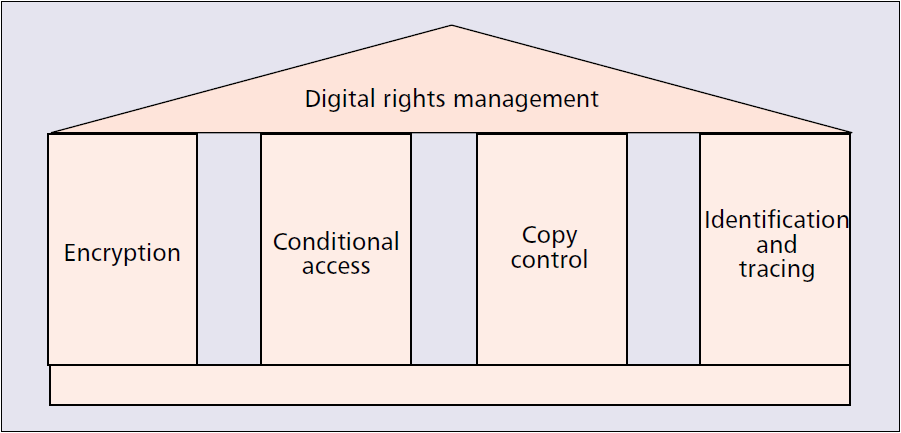
\includegraphics[width=13cm]{drm_pillar}
   \caption{The DRM pillar model (Copied from Hartung and  Ramme (2000) \cite{ieee:drm_watermark}).}
   \label{fig:def:drm_pillar}
\end{figure}
At large, the DRM regroups many technologies that will typically:
\vspace{-17pt}\begin{itemize}
	\item Authenticate and identify the user and/or its devices to make sure the content is accessed and consumed by authorized person. The \textquoteleft Copy control\textquoteright ~pillar in figure \ref{fig:def:drm_pillar}.
	\item Protect and encrypt the content to avoid third party access. The \textquoteleft Encryption\textquoteright ~pillar.
	\item Make each copy unique in order to identify them and track their usage. The \textquoteleft Identification and tracing\textquoteright ~pillar.
	\item Define and enforce the license such as if the user can copy the text, print it, limit the number of device that can access it, set the access duration (e.g. for library lending), if the copy can be shared and how many times, etc. The \textquoteleft Conditional access\textquoteright ~pillar.
\end{itemize}

\begin{figure}[h]
   \centering
   	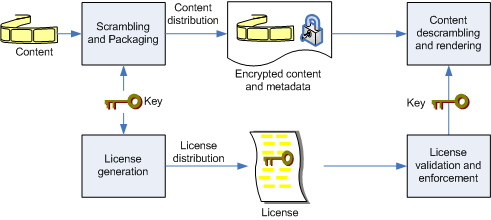
\includegraphics{indicare_drm}
   \caption{A generic DRM system (Copied from Maru\v{s}i\v{c} et al. (2005) \cite{indicare:tiramisu}).}
   \label{fig:def:drm_scheme}
\end{figure}

A DRM system is presented in figure \ref{fig:def:drm_scheme} where \textquotedblleft the privilege to consume protected content is granted to the end-user by a license, which specifies usage terms and conditions and includes the key(s) needed for content descrambling\textquotedblright ~\cite{indicare:tiramisu}. In more details, on the provider side, once the user purchases content, a key is generated based on user identifier. This key will be used to sign (make the copy unique) and encrypt (protect) the file (the \textquoteleft Scrambling and Packaging\textquoteright ~box). In parallel, the usage contract (\textquoteleft License generation\textquoteright ~box) is issued. After these steps, the encrypted content and the license is delivered to the user. On the user device, if the reading application is legitimate and will satisfy and enforce the license (\textquoteleft License validation and enforcement\textquoteright ~box), the key is used to decrypt the file and the content is now displayed to the user (\textquoteleft Content descrambling and rendering\textquoteright ~box).


But even with strong encryption and/or full control on the software and hardware, there will always be people with computer skills that will find a way to break any technical measure.\label{def:law_intro} To hamper software cracking to be implemented, distributed and used for protection removal, new articles were added in the international copyright treaty (the law is described in section \ref{def:law_drm}) to make such crack illegal in order to have the DRM effective.

Daniels use the term \textquotedblleft \textbf{hard DRM}\textquotedblright ~\cite{dan:hard-soft-drm-1} to describe the DRM system that \textquotedblleft restricts physical access and usage of the file\textquotedblright. Rosenblatt describes it as \textquotedblleft \textbf{heavyweight DRM}\textquotedblright ~\cite{idpf:lcp-uc}. With that definition, he can introduce the \textquotedblleft \textbf{lightweight DRM}\textquotedblright ~concept which can be compare to the \textquotedblleft PDF [\ldots] password-based encryption\textquotedblright . With the \textbf{password protection} approach, there is no need to call back a distant server for authentication/authorization since the protection is embedded within the file. The key to decrypt the file is a password that the user has to enter before he can access the content. Like with hard DRM, this technique can also manage the usage such as restricting printing, limiting copy of content, etc. Usually, because there is no communication with a central authentication, this technology will not block concurrent access nor limit the number of devices which host copies of the file. \label{def:password_protection}

\section{Social DRM, Watermark, Fingerprint}

\textbf{Watermark} or \textbf{fingerprint} can be used to identify a file. They originate from the information hiding techniques. Petitcolas et al. classify them as \textquotedblleft robust copyright marking\textquotedblright ~\cite{ieee:info_hiding} as shown in figure \ref{fig:def:drm_finger}. The watermark\label{def:watermark} consists of data (for example, the name and credit card number of the person who purchase the file) that are inserted and hidden inside the file bytes as well as imperceptible changes to the content (like spaces and invisible characters at the end of the chapter, modify pixels of the font, change the line/text spacing (see figure \vref{fig:def:drm_watermark})) and many other (such as modifying the file name, using digital steganography (e.g. apply to the cover image), etc.). One important aspect is the number of different watermark techniques used, so the cracker can never be sure to have defeated them all.
\begin{figure}[h]
   \centering
   	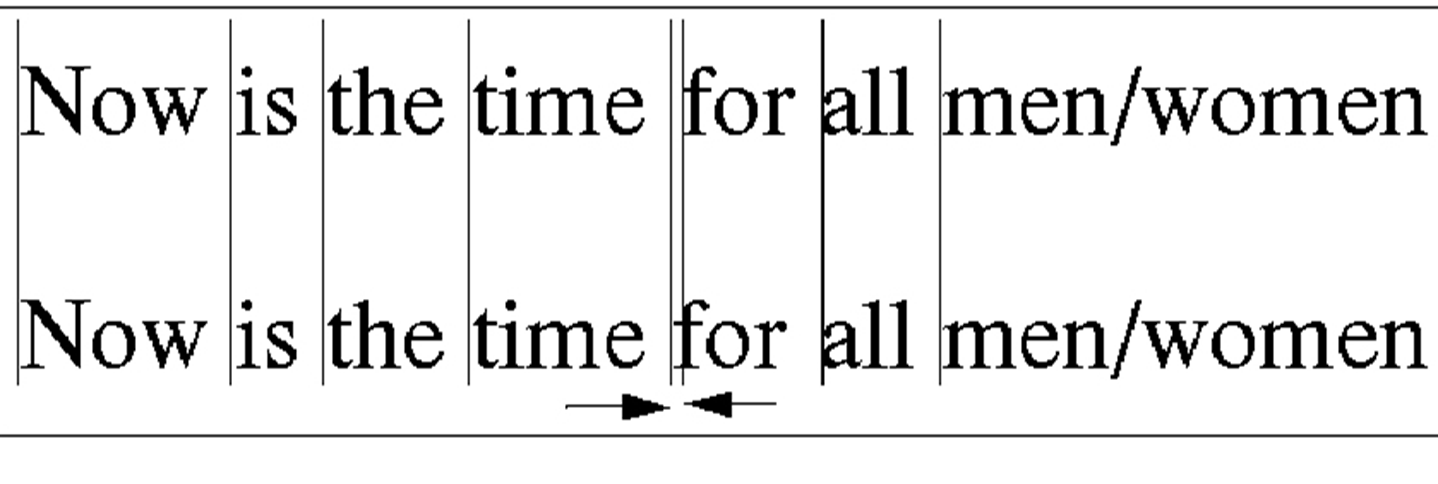
\includegraphics[width=11cm]{watermark}
   \caption{Word-shift watermark example (Copied from Lee (2001) \cite{lee:watermark}).}
   \label{fig:def:drm_watermark}
\end{figure}

Fingerprint is a technique to uniquely identify a copy of a file by generating a cryptographic hash. These techniques can be used to do a a posteriori protection. Because it does not control the permission, so the user can do whatever he want with the file; here the idea is to be able to find the user if he did something unlawful (for example, distribute copies of the file on peer-to-peer network).
\begin{figure}[h]
   \centering
   	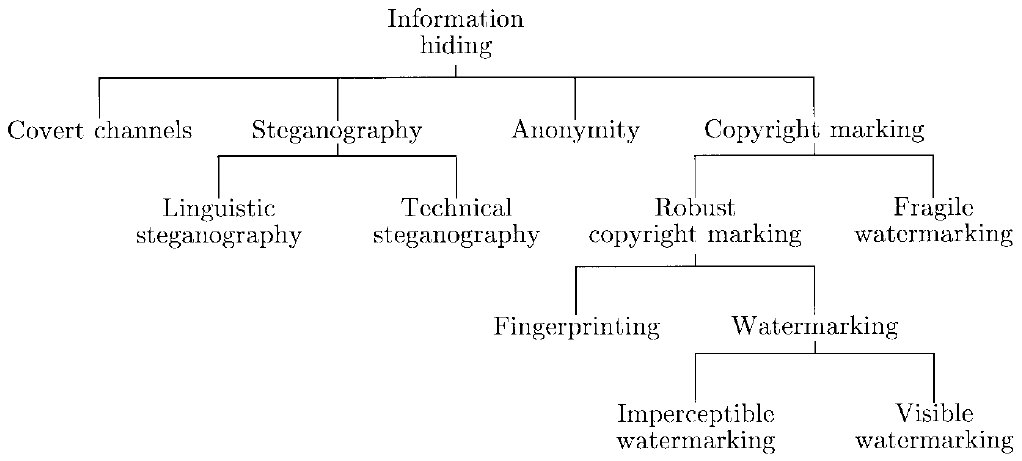
\includegraphics[width=11cm]{information_hiding}
   \caption{A classification of information-hiding techniques (Copied from Petitcolas et al. (1999) \cite{ieee:info_hiding}).}
   \label{fig:def:drm_finger}
\end{figure}

A similar approach to watermark is \textbf{social DRM}\label{def:social_drm}. The difference is that the information about the user is not hidden but is visible. For example, be part of meta-data or simply visible in plain text e.g. in the footer of every page or as in figure \ref{fig:def:drm_socialDRM} where the PackaDRM\texttrademark ~presents the user information in the \textquoteleft terms and conditions\textquoteright. The idea here is to let the user do what he want but putting pressure on him to not do anything illegal. 
\begin{figure}[h]
   \centering
   	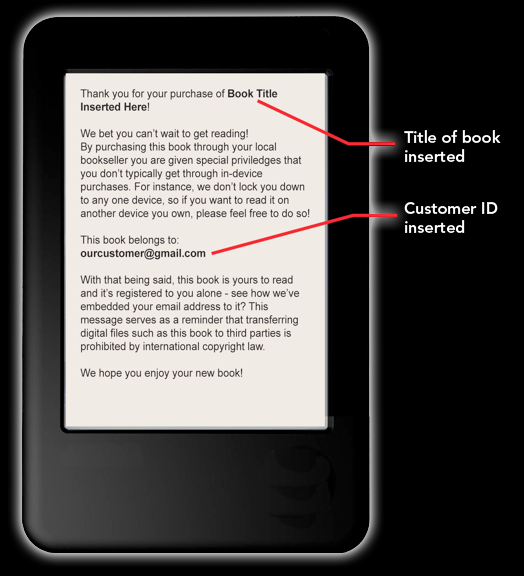
\includegraphics[width=11cm]{PackaDRM}%
   \caption{Social DRM (Copied from Franco (2012) \cite{kevinfranco:socialDRM}).}
   \label{fig:def:drm_socialDRM}
\end{figure}

The watermark and all the others identification technologies can and are often used in combination with the DRM. For example, Rosenblatt specifies that the Lightweight DRM \textquotedblleft is intended to be complementary to watermarking\textquotedblright ~\cite{idpf:lcp-rfp} or as Hartung and Ramme state \textquotedblleft watermarking [\ldots] is only useful as a system component, with the most important application being DRM and copyright protection in general\textquotedblright ~\cite{ieee:drm_watermark}. Daniels refers to the combination of social DRM and watermark as \textquotedblleft \textbf{soft DRM}\textquotedblright ~\cite{dan:hard-soft-drm-2} in the sense that \textquotedblleft it is \textquoteleft soft\textquoteright ~in that it is not enforced by technology, only law\textquotedblright.


\section{Protection in the Law}\label{def:law}

In order to have the protection effective and to make the crack illegal, the World Intellectual Property Organization\footnote{The WIPO is an United Nations (UN) agency established in 1967 which is responsible for the use of intellectual property (such as copyright, patents, trademarks, etc.) and count 185 member states (from: \url{http://www.wipo.int/about-wipo/en/}).} (WIPO) has added measures to protect DRM in its WIPO Copyright Treaty (WCT) of 1996 \cite[articles 11 and 12]{wipo:wct}. These articles are enacted in the European Union (EU) in the DIRECTIVE 2001/29/EC OF THE EUROPEAN PARLIAMENT AND OF THE COUNCIL of 22 May 2001 on the harmonisation of certain aspects of copyright and related rights in the information society \cite[chapter III]{eur-lex:2001/29/EC} implemented in Finland under the COPYRIGHT LEGISLATION of 2010 \cite[chapter 5a]{finlex:copyright_act}. Under the 89 WCT contracting parties such as China, Japan, Canada, Russian Federation, let mention the United States of America who enacted this treaty under the Digital Millennium Copyright Act of 1998 \cite[section 103]{gpo:dmca}. Notice also that countries such as India or Brazil are not signatories of the WCT.

\label{def:law_drm}In the WCT \cite[article 11]{wipo:wct}, EU DIRECTIVE 2001/29/EC \cite[article 6]{eur-lex:2001/29/EC} and Finnish COPYRIGHT ACT \cite[sections 50a and 50b]{finlex:copyright_act}, removing, circumventing any effective technological measures (such as hard and lightweight DRM), providing or producing tools to remove or circumvent it are prohibited. Finnish COPYRIGHT ACT  specifies that anyone who circumvent DRM, produce or distribute tool or device for circumventing a technological measure \textquotedblleft shall be sentenced [\ldots] to a fine for a violation of a technological measure\textquotedblright ~\cite[section 56e]{finlex:copyright_act} and \textquotedblleft shall be obliged to pay the author damages for any loss, mental suffering or other detriment caused by the crime\textquotedblright ~\cite[section 57(3)]{finlex:copyright_act}.

\label{def:law_watermark}The WCT \cite[article 12]{wipo:wct}, EU DIRECTIVE 2001/29/EC \cite[article 7]{eur-lex:2001/29/EC} and Finnish COPYRIGHT ACT \cite[section 50d]{finlex:copyright_act} make removing or altering right management information or distributing, importing for distribution, broadcasting, communicating or making available to the public a work from which electronic rights-management information has been removed or altered illegal. The Finnish COPYRIGHT ACT \cite[chapter 7, sections 56f and 57(3)]{finlex:copyright_act} specifies the same type of punishment as for circumventing a technological measure.

The WCT \cite[article 12(2)]{wipo:wct} defines right management information as \textquotedblleft information which identifies the work, the author of the work, the owner of any right in the work, or information about the terms and conditions of use of the work, and any numbers or codes that represent such information\textquotedblright . To make sure that the social DRM belong to that definition, part of it should be placed in under the copyright notice and/or under the terms and conditions section of the e-book. Another possibility could be, for example, to have a book ID (which identifies the work) with a reminder to the user that this information is stored with his purchase detail in reseller database. 

The watermark represents right management information; but by being invisible would not match the definition. Even if the terms and conditions forbid to remove it, \textquotedblleft it is possible that copyright law may prevail over such terms; this is a legal gray area\textquotedblright ~\cite{rosenblatt:pottermore}. Another problem with watermark that Rosenblatt raises: \textquotedblleft a lightweight DRM that is susceptible to one-click crack has more protection than, say, a watermark removal tool\textquotedblright ~\cite{idpf:lcp-uc}. So a watermark removal tool is legal  because the watermark can not be considered as an effective technological measures, while a DRM removal tool is illegal. This non-fully law protection could be one more argument to use watermark only in combination with other protection techniques or as Hartung and Ramme state \textquotedblleft watermarking is not a standalone technology\textquotedblright ~\cite{ieee:drm_watermark}. 


\chapter{E-book File Formats and Protection}

For e-book there are different file formats available with their qualities and limitations.


The most basic file format is the plain text (usually with extension .txt) which has the advantage of being universal, i.e. can be read on any operating system, even in command line environment and with an external tool can be compressed with a good rate for transport, e.g. through internet; but will take its full size on disk because it must be uncompressed before reading. This format was designed to display text only, that can be a limitation for e-book because of a poor formatting such as no bold or italic text, impossible to insert images, interactive links, etc. And finally almost no content protection; with administrator privilege, the end user can easily copy the full text and modify it.

\label{def:e-book:pdf}In 2008, after seventeen years of existence, the portable document format (.pdf) became a standard. It has always been a popular format on the internet for document exchange and also for the e-book (according to a French survey \cite[p. 19]{OpinionWay:baro_v1}, it is the preferred format for 53\% of the readers). By being a standard, every operating system can have application to display and print files in this format. It proposes many text formatting options, allows insertion of links and pictures, supports interactive (form) and multimedia (audio, video) elements. This format was designed to be page oriented where the electronic version is the same as its print equivalent (this is sometimes seen as a problem, especially on small screen) but supports also re-flow feature. At the protection level, the author of the file can allow or deny the printing, copying of content, page extraction, etc. and the file can be secured by password or be electronically signed (Adobe DRM is detailed in subsection \vref{def:adobe_drm})~\cite{adobe:pdf}.

\label{def:e-book:epub} Another open standard file format widely use for e-book is EPUB (for electronic publication (with .epub file extension)) standardized in 2007 which is the successor of the Open eBook (OEB) format of 1999 \cite{idpf:epub}. As of 2012 its latest version is EPUB 3.
 
EPUB format uses web standards like hyper text markup language (XHTML (in EPUB 2) or HTML 5 (in EPUB 3)) files representing the text and structure, cascading style sheet (CSS) for the formatting, an opf file based on extensible markup language (XML) for the navigation and additionally images, sounds, videos, etc. ~all together compressed into the EPUB file. 
This native compression is advantageous for the device disk usage and for faster transmission. 
The other big difference with the PDF is the use of the dynamic layout and pagination of the HTML so the text will be adapted on the fly to the display area and the user preferred font size \cite{idpf:epub3}. 

\label{def:e-book:epub-drm}The EPUB file format offers a protection layer but \textquotedblleft does not specify a required format for DRM\textquotedblright ~\cite[section 2.5.5]{idpf:ocf_spec}; so the choice is in the hands of the publisher/vendor. As example, the Adobe DRM (see \vref{def:adobe_drm}) can be use to protect EPUB files. However, the International Digital Publishing Forum (IDPF)\footnote{IDPF is the organization responsible to maintain the EPUB standard.} is proposing \textquotedblleft requirements for a potential content protection scheme for EPUB\textquotedblright ~\cite{idpf:drm-rfc} (lightweight DRM is extended in section \vref{def:idpf_light}).

\label{def:e-book:iba:azw} TODO amazon, ibook, lit
In 2000 Mobipocket.com developed their own e-book file format (with a .mobi or .prc file extension) as part of their MobiPocket Reader application. This format, like ePub, is based on the Open eBook (OEB) specifications. The file can be natively secured with their solution but also left unencrypted. Mobipocket became part of Amazon in 2005. \cite{mobi:about}

After Amazon acquisition, they build there own protection on top of the Mobipocket format (with a .azw extension). This has made the future of the protected .mobi e-book unclear \cite{tdr:rip_mobi} while unprotected .mobi files can still be read from Amazon Kindle devices as well as many reading applications. Amazon also announced the creation of their new Kindle Format 8 (with a .kf8 or .azw3 extension) based on HTML 5 and CSS 3. Like the .azw, it can be protected with Amazon DRM. This format should continue to be backward compatible with Mobipocket (.azw and also unencrypted .mobi). The .azw and .kf8 e-books can only be read from Amazon Kindle devices or with Amazon Kindle Reading apps\footnote{\url{http://www.amazon.com/gp/feature.html?ie=UTF8&docId=1000493771}} for Microsoft Window, Mac, mobile phone and tablet\cite{amazon:kf8}.

Apple also has its own e-book file format (with a .iBooks or .iba extension) based on EPUB 3 but with their own \textquotedblleft mimetype and proprietary CSS extensions\textquotedblright ~\cite{glaz:iba}. The e-books in this format can be protected by Apple DRM and if obtain through their store will anyway be watermarked. This format is designed to be only readable with the iBooks application\footnote{\url{https://itunes.apple.com/us/app/ibooks/id364709193?mt=8}} and only on Apple mobile devices. For an author/publisher, the only way to sell e-books in this format is through the Apple store \cite{apple:iba_faq}. 

 


\chapter{Existing and Upcoming Technologies}

\section{Existing E-book DRM}

Nowadays, there is four major e-book DRM in use one each from Adobe, Amazon, Apple and Marlin Trust Management Organization (MTMO). Adobe e-book DRM will be described in detail in section \vref{def:adobe_drm} since it is among the few that gives details on their solution; the other being the MTMO\footnote{\url{http://www.marlin-community.com/technology/how_marlin_works}}. For Amazon and Apple, it is hard to find information on their DRM system because they use it only on their respective platform. So, by not communicate about it, that help them in protecting their DRM technologies.

The Microsoft e-book DRM technology can not be considered in use since it was part of the Microsoft Reader that has been discontinued in August 2012 (see section \vref{def:opp_ms}). Microsoft will probably use their PlayReady\footnote{\url{http://www.microsoft.com/playready/}} technology to protect e-book. Their white paper specify that \textquotedblleft Microsoft PlayReady supports essentially any type of content, including games, images, and ringtones, in addition to music and video.\textquotedblright ~\cite[p. 4]{ms:playready}; but don't explicitly have the e-book in the list. 

\subsection{Adobe DRM in Detail}\label{def:adobe_drm}

Adobe e-book DRM, namely Adobe Digital Experience Protection Technology (ADEPT), is part of their platform which is center around the Adobe Content Server\footnote{\url{http://www.adobe.com/products/content-server.html}} which serves as both hosting and managing PDF and EPUB e-books distribution (see figure \vref{fig:def:adobe_workflow})
\begin{figure}[h]
   \centering
   	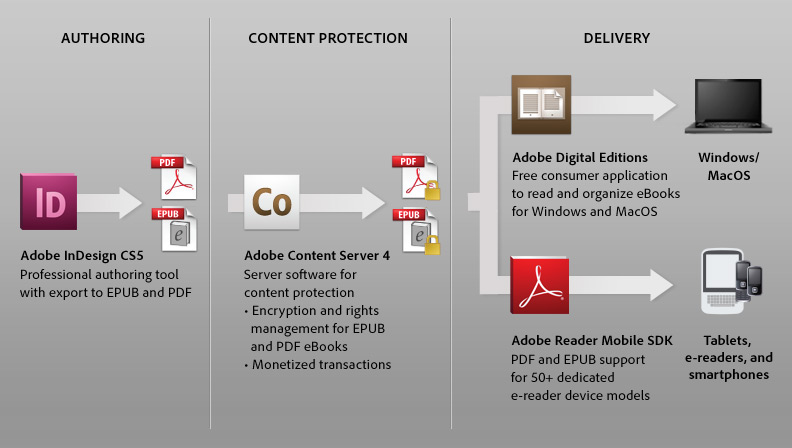
\includegraphics[width=14.7cm]{adobe_ebook_workflow}
   %
   \caption{Adobe Digital Publishing Solution for eBooks (Copied from Adobe (2012) \cite{adobe:digital_publishing}).}
   \label{fig:def:adobe_workflow}
\end{figure}
in conjunction with the Adobe Digital Editions\footnote{\url{http://www.adobe.com/products/digital-editions.html}} software for Windows or Mac, or an application written with the Adobe Reader Mobile Software Development Kit (SDK)\footnote{\url{http://www.adobe.com/devnet/readermobile.html}} for e-reader device, tablet or smart-phone that will provide to the user the way to access the protected files \cite{adobe:whitepaper}.

In the normal flow (see figure\vref{fig:def:adobe_cs}), the user visits the publisher or retailer web store to buy an e-book (or a library website to borrow an e-book). After the money transaction (or entering his library credential), he will receive an Adobe Content Server Message (.acsm) file and by opening it with the Adobe Digital Editions, the software will communicate on-line with the publisher/retailer/library's Content Server that will encrypt the e-book and provides it DRM protected with the publisher's authorizations (like allow/deny printing, copying text, duration of validity, etc.) for the user based on his adobe ID.
\begin{figure}[h]
   \setlength{\fboxsep}{3pt}
   \fbox{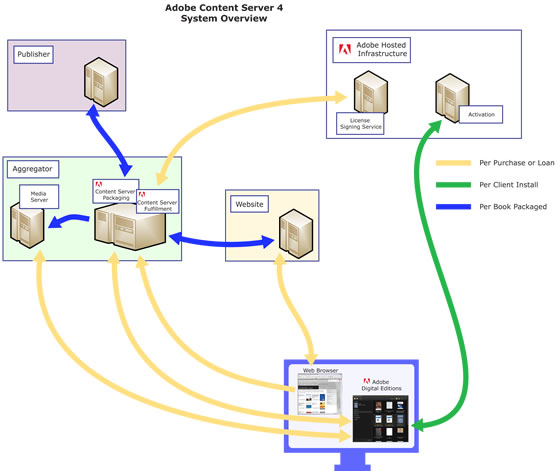
\includegraphics[width=14.7cm]{adobe_cs4-overview}} 
   \caption{Adobe Content Server Architecture (Copied from Adobe (2012) \cite{adobe:content_server_architecture}).}
   \label{fig:def:adobe_cs}
\end{figure}
Before the user can read the e-book, he must also have registered his device. That way, the platform makes sure that the file owned by the user is not distributed further. 

But to be fair, Adobe DRM system allows the user to register up to 6 devices\label{def:adobe_limit}, so the user can access his library, annotations, bookmarks, etc. on all of them, e.g. start to read on his e-reading device, continue on his smart-phone and finish on his laptop. This can also cover the family fair use where people share a home computer.

\subsection{Advantages and Limitations of Adobe DRM}

One natural thing that user can do with physical books is to share it with friends. 
Unfortunately, Adobe DRM do not allow it since the e-book is DRM protected for the user and its devices only. 
In order to give sharing facility Adobe offer another way to provide the e-book to the user with a password-only protection \cite[Ability to share section]{adobe:whitepaper}. 
The password will be encrypted with the file and it will be impossible to modify it. 
The publisher can choose to let the user define it and allow a open sharing.
%vref bug?
Or use a social DRM (see section \ref{def:social_drm} on page \pageref{def:social_drm}) like approach where the publisher create the password for the user (e.g. using user credit card number, email address, etc.) to refrain the user to share it worldwide. 
And this password-only protection option is at the goodwill of the publisher, so the sharing with Adobe DRM is still very weak.

One advantage of Adobe e-book DRM compare to Amazon and Apple is that the user is not imprisoned in a walled-garden system and can purchase DRM protected e-books and/or borrow from different vendors/libraries and can aggregate, organize and read them within the same application. Apple iBookstore allows only iOS ($\geqslant$ 4) devices, namely iPad, iPhone and iPod Touch to purchase files from their store and also prevent them to get e-books from a retailer who use a different DRM in their iBooks application. And to finish the Apple close loop, e-book created from their iBooks Author tool can only be sold through iBookstore \cite{zdnet:apple_ibooks_license}. Amazon Kindle device also lock the user with a single vendor. But by reading Adobe white paper carefully \cite[Open environment section]{adobe:whitepaper}, their argument is that many vendor use their DRM making the multiple vendors aggregation possible; but the Adobe Digital Editions will also fail to open a e-book encrypted with another DRM.

For publishers/authors, another advantage of Adobe DRM approach is the use of the open and well known formats PDF (described in \vref{def:e-book:pdf}) and EPUB (see \vref{def:e-book:epub}), in opposition to the proprietary format from Apple iBooks and Amazon Kindle (as described in \ref{def:e-book:iba:azw} on page \pageref{def:e-book:iba:azw}), thus simplifying the production, publication and distribution process \cite[How the Adobe eBook Platform helps publishers section]{adobe:whitepaper}. For the reader however, the advantages of these open format get reduced. As example, the DRM force the user to use the Adobe Digital Editions, preventing him to use his favourite EPUB/PDF reading application and can thus create some confusion.
%vref bug again: \vref{def:e-book:iba:azw}

Another claim of the Adobe whitepaper \cite[Device interoperability section]{adobe:whitepaper} is the possibility to read DRM protected e-books on multiple platform. In fact, Adobe provide only the computer support with their free\footnote{Free here has the meaning of gratis/no price.} Adobe Digital Editions application for Windows and MacOS Operating systems, excluding GNU/Linux \cite{adobe:ade_linux}. For the other devices/platform, the e-book vendor or a third party has to develop a dedicated application using the Adobe Reader Mobile SDK, for which they have to pay a licence. Even if the price is fixed on a case-by-case basis, this can be unfair for a small publisher and is seen as another way from Adobe to monetise their DRM.

As the DRM secret-holder, Adobe has freehand for the price politic. 
Concretely, in 2008, the license for the Adobe Content Server was \$5000\footnote{United States dollar (USD)} plus an extra \$1500 per year for the support, maintenance, upgrade and the access to the Digital Signing Service \cite{adobe:content_server_price}. 
And now in 2012, from the Adobe Technology Partner in Europe \cite{ctrlpublishing:content_server_price}, 
the license is \$8000 plus \$2000 per year support. 
They also charge \$2495 for the installation and configuration. 
On top of that price, signing one e-book permanently will cost \$0.22 (\$0.08 for a 0-60 day expiring (e.g. for a library lending)). 
If such price is affordable for a big publisher, it can be too much for a small one.
\begin{figure}[h]
   \setlength{\fboxsep}{3pt}
   \fbox{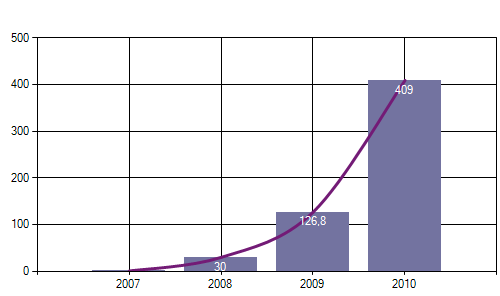
\includegraphics[width=14.1cm]{e-book-sales-finland}}
   \caption{Downloaded e-books total. Yearly sales (1000 \euro) 2007-2010 in Finland. 
   (Copied from Finnish Book Publishers Association (2012) \cite{kustantajat:year_sale_ebook}).}
   \label{fig:def:e-book-sale-fi}
\end{figure}

As example,\label{def:e-book-sale-fi} based on the yearly sales in Finland (see figure \ref{fig:def:e-book-sale-fi}), even if the progression is about 30\% per year, it can be reasonable to say that a publisher sell ten thousand e-books per year. If he want to cover the license and installation (e.g. over a three year period) price, the yearly fee plus the 22 cents per e-book, he would have to charge an extra \$0.77 per e-book he sell (and that do not include other charges for maintaining a server (like hardware/software installation and maintenance, electricity, domain name and internet address, etc.)).
%vref bug :(

In the others limitations, it is impossible for a user to offer or resell his e-books (or at least this information is totally hidden from Adobe). Due to the fact that the DRM is attached to the user and the device, it will be hopeless to try to read an e-book on a public computer (e.g. in an internet coffee). Also, if the user reach the limit of the 6 registered devices, buy a new computer and want an old one to be unregistered to replace it with his new one, he will face a unpleasant procedure to do so.

And as any technical measure, it was just a matter of time, about two year after the release of the Adobe Digital Editions that the explications on how to circumvent the Adobe ADEPT DRM was published \cite{icabbages:adobe_drm_hack} on the I$\heartsuit$\textsc{cabbages} blog\label{def:adobe_drm_crack}. The author specifies that the Adobe file encryption was strong but the weakness was in how the Adobe Digital Editions hide the key. Nowadays, there is even companies like the epubor \cite{epubor:adobe_drm_removal} that do business by selling DRM removal tools. 


\section{Lightweight DRM}\label{def:idpf_light}

In May 2012, IDPF made a proposal for standardizing a Lightweight Content Protection (LCP) that will be \textquotedblleft occupying a middle ground between strong DRM and DRM-free\textquotedblright ~\cite{idpf:drm-rfc} to protect EPUB e-books (see section \vref{def:e-book:epub-drm}).
The idea is to have a protection that will be strong enough to qualify as a \textquoteleft effective technical protection measure\textquoteright ~to benefit the law protection (as explained in \vref{def:law_drm}) to guarantee the publisher/vendor with a full DRM mechanism and at the same time reduce the \textquoteleft hard DRM\textquoteright ~drawbacks (see section \vref{def:opp}) \cite{idpf:lcp-uc}.

The LCP will work as follow: when a reader acquires an e-book, the content (texts, images, etc.) will be encrypted with a password protection and the hash of the password will be associated with the file and/or the reading application. So, to read the e-book, the user will be prompted to enter it the first time before accessing the content. Since the password can not be changed and will be set at purchase time, it can be define by the vendor/publisher (to be e.g. the reader full name, email address, credit card number, etc.) \cite{idpf:lcp-uc}.



\subsection{Advantages and Limitations of Lightweight DRM}

A first argument for the IDPF is to make LCP a standard. This way, it will allow more devices and reading applications to be able to open and display the protected content, ensuring better interoperability. The reader would enjoy acquiring and reading e-books from different vendors/publishers using his favourite application/device, thus reducing the market fragmentation or lock-in \cite[Why Consider LCP for EPUB? section]{idpf:lcp-uc}. However, the same document also states that \textquotedblleft the resulting EPUB LCP [\ldots] would likely be published under licensing regimes. [\ldots] Use of the technology would be expected to be charged on a cost recovery basis.\textquotedblright ~\cite[What Is the Recommended Process For Defining LCP for EPUB? section]{idpf:lcp-uc}. So the risk is that some application/device providers will refuse to implement the LCP and/or some e-book vendors would continue to use other DRM systems and ignore LCP.

With the password protection, there is no need to communicate with a distant authentication server, so LCP will work offline and it also means that the reader will really own the e-book (as long as he remembers the password) even if the provider ceases its activities. He will also have the freedom to have copies of his e-books on any devices he owns without limitation. 
The reader will be able to share his e-book; but will have to communicate the password too, so limiting him to people he trusts (friends/family) and refrain him to over-share it.
And finally LCP will better respect user privacy by not spying the reader usage \cite[Why Consider LCP for EPUB? and What Is LCP? sections]{idpf:lcp-uc}.

With the content encryption, the publisher/vendor can also define limitation on usage like printing, copy of content, editing, etc. There will be also a possibility to set a expiration date which can be interesting for library lending. Basically, the provider will be able to set the same type of protection that he can do with other DRM \cite[EPUB LCP Requirements section]{idpf:lcp-uc}.

By being lightweight, it means that the implementation cost will be reduced. For the user device, less power and memory will be required, a fast decryption process and no communication with a distant server \cite[What Is LCP? section]{idpf:lcp-uc}. For the provider, it will only need a simple signing/encryption mechanism, for example trough a web service without needing a complex server architecture \cite[What Is LCP? and Requirements sections]{idpf:lcp-rfp}. However, the cost in term of price as well as the licensing will be addressed later \cite[Requirements section]{idpf:lcp-rfp}, which makes it unclear how much it will really be. And also, there are known patents\footnote{e.g. intertrust holds over 200 patents in the digital media protection field (from: \url{http://www.intertrust.com/technologies/patents})} that exist, so a risk to have to pay royalties to third parties as an extra cost for the LCP implementation.

IDPF is aware of some possible weaknesses. First, the LCP, like any DRM, will be cracked. But, they count on the anti-circumvention law (see section \vref{def:law_drm}) to have some level of crack protection \cite[What Is LCP? section]{idpf:lcp-uc}. While modern DRM have some possibilities to recover and resist to crack, the LCP will not benefit from such features and because it is designed to not spy on the user, it means that it is not possible to monitor user activities such as suspicious ones \cite[What Is LCP? section]{idpf:lcp-rfp}. 
The others weaknesses concern the impossibilities to have some business model such as \textquotedblleft Domain authentication\textquotedblright, \textquotedblleft License chaining\textquotedblright, \textquotedblleft Master-slave schemes\textquotedblright ~and \textquotedblleft Forward-and-delete\textquotedblright ~models \cite[What Is LCP? section]{idpf:lcp-rfp}.

Another concern is how will the IDPF deals with free\footnote{free as in freedom.} reading software licensed under the GNU General Public License Version 3 (GPLv3) such as Calibre\footnote{Calibre is a e-book reading application that also offers other tools such as library management, synchronization with multiple devices, e-book file conversion, etc. (from: \url{http://calibre-ebook.com/about})}. The GPLv3 under the point 3 of the terms and conditions state that \textquotedblleft [\ldots]you waive any legal power to forbid circumvention of technological measures[\ldots]\textquotedblright ~\cite{fsf:gplv3}, in other words, anyone with programming skills would legally have the right to modify the Calibre software to e.g. add a feature to \textquoteleft save the EPUB e-book unencrypted\textquoteright ~and the right to distribute such modified version of the application. So will IDPF forbid free application to implement the LCP and in doing so, loosing the interoperability? Or will they allow such software to implement LCP, knowing that the protection can legally be nullified?

Finally, there is no clear date when the LCP will be released. In the use cases and requirements, it only states that \textquotedblleft IDPF solicit contributions of existing technology that could become the basis of a market-relevant solution for LCP within the next 12 calendar months or less\textquotedblright ~\cite[Why Consider LCP for EPUB? section]{idpf:lcp-uc}, meaning something around mid 2013? And also that IDPF envisions the possibility that there can be no LCP at all: \textquotedblleft [\ldots]it does not represent any commitment by the IDPF to establish a solution. [\ldots] it may become clear that no feasible standardized solution would be sufficiently useful or accepted, or that no solution is forthcoming that will sufficiently address critical requirements.\textquotedblright ~\cite{idpf:drm-rfc}.

\chapter{No Control}

\section{DRM Opponents and Limitations}\label{def:opp}

The opponent to the DRM, such as the Free Software Foundation (fsf) through their \textquoteleft defective by design\textquoteright ~campaign define DRM as \textquotedblleft Digital Restriction Management\textquotedblright ~because they see it as restricting the fair use like limitation of the private copies and backup, makes hard or impossible to share, swap, offer or resell purchased files.
It also imprison the user in non-free\footnote{Free here has the meaning freedom/liberty in opposition to proprietary (so nothing related to the price/cost).} reading software where the user is forced to agree with policy (that may downgrade his rights with new software upgrade) otherwise he looses his files. They also raise privacy concerns where such software can monitor user computer's hard disk and spy his usage. They finally denounce a back-door that allow vendor to remotely delete the e-books form the devices of the users; with the example of Amazon removing the George Orwell 1984 e-book from hundreds of users\footnote{http://www.defectivebydesign.org/blog/1248} or more recently clearing the full collection from one reader\footnote{http://www.defectivebydesign.org/node/2250} \cite{fsf:defectivebydesign}.

Even if the EU DIRECTIVE 2001/29/EC \cite[article 6(4)]{eur-lex:2001/29/EC} request that the DRM respect some of the exceptions (from \cite[article 5]{eur-lex:2001/29/EC}); it makes for example optional the private copy and as such, in the Finnish COPYRIGHT ACT \cite[section 50c(1)]{finlex:copyright_act} this exception is not present; so in Finland, a DRM can legally forbid the private copy that confirm the fsf concerns. There are many others fair uses that may be restricted by DRM such as reproduction by the press, communication to the public \cite[article 5(3)(c)]{eur-lex:2001/29/EC}, use for purpose of caricature, parody or pastiche \cite[article 5(3)(k)]{eur-lex:2001/29/EC}, use during religious celebration \cite[article 5(3)(g)]{eur-lex:2001/29/EC}, etc.

Others complain that the DRM is more a protection for the services of the provider than a protection of the copyright \cite[chapter 7]{droit-technologie:internet_copyright}. The exceptions, that DRM must follow, concern almost only public institutions (libraries, schools, museums, hospitals or prisons) and thus can be unfair for a private user. An example: A private user want to copy part of the text of a DRM protected e-book for a quotation with purpose of review \cite[article 5(3)(d)]{eur-lex:2001/29/EC} and if the DRM restrict the copy of the text, he would have to circumvent it to reach his goal. So he will not infringe the copyright law; but he will be guilty for circumventing a technological measure. While if he was removing the DRM to distribute unauthorized copies, he would already violate the copyright; so the DRM is not playing its role, except that now the user will be punished twice for infringing the copyright and the technical measure.

Because DRM can limit the number of devices (see section \vref{def:adobe_limit}) the user can use to read his e-book and by knowing that the user will probably buy a new device every year or two, it means that he will have problems when he reaches that limit. He will not understand that he was paying for a service instead of owning his files. This will also stops the social sharing (e.g. to lend an e-book to his friends or family members) restricting one aspect of the reading experience.

The Electronic Frontier Foundation (EFF) shares the same type of concerns that the fsf. EFF goes further against big companies by stating that the DRM is an anti-competitive practice \cite{eff:drm}. \label{def:opp:anti-competitive} As example, if the vendor proposes the e-book in a single protected proprietary file format, forcing the reader to access it only with a specific hardware and/or software, that will forbid the user to access DRM protected content from a concurrent with the same device/application; it will lock the user to a single vendor. That type of strategies are seen from Amazon, Apple and some others. In the other side, if the publisher impose protection, a small reseller will have problem to pay for a DRM system (see example in section \vref{def:e-book-sale-fi}); clearing the market for the big companies. For Doctorow \cite[chapter 28]{doctorow:context}, the protection does not benefit the writer nor the publisher nor the end user but put the power in the hands of the DRM provider.

EFF also says that \textquotedblleft putting DRM on e-books is short-sighted, futile, and doomed\textquotedblright ~\cite{eff:e-book_drm_fail}. 
\begin{figure}[h]
   \centering
   	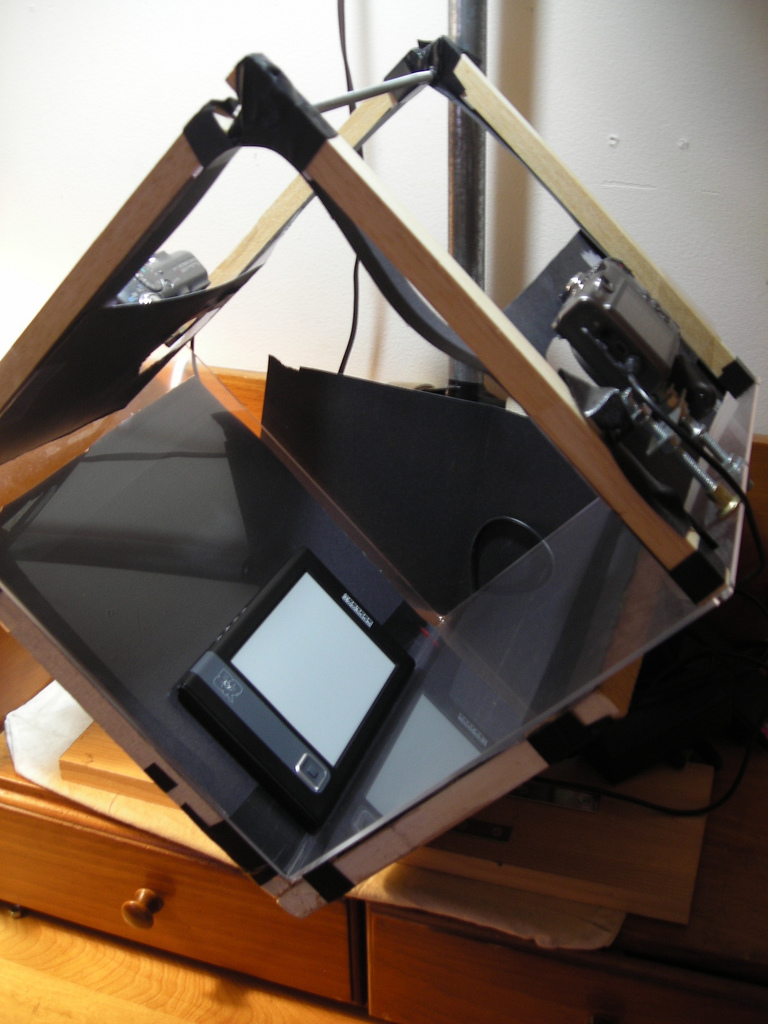
\includegraphics[width=7.1cm]{flickr_e-book-ripper}
   \caption{e-book ripper (Copied from bkrpr.org (2009) \cite{flickr:e-book_ripper}).}
   \label{fig:def:e-book_ripper}
\end{figure}
Basically, the best e-book DRM will suffer from the analog hole. In other words, the protection ends once displayed on screen. So anyone with a digital camera and an Optical Character Recognition (OCR) software can get an almost perfect DRM-free copy in few minutes. As example, in figure \ref{fig:def:e-book_ripper}, a book ripper normally design to digitalize physical book\footnote{Where the book is placed in the middle and when turning every pages, take a picture of the odd page with the left camera (the right one for the even page). When the end of the book is reach, the pictures are treated with an OCR software that will produce the e-book.} is used to free up a DRM protected e-book from a reader device. 

An other fear for the user is if the vendor goes bankrupt or if the DRM provider stops to maintain the system. This happens with Microsoft\label{def:opp_ms} announcing that they will not support any more the .lit file format: \textquotedblleft Microsoft is discontinuing Microsoft Reader effective August 30, 2012, which includes download access of the Microsoft Reader application from the Microsoft Reader website\textquotedblright ~\cite{microsoft:reader}; so the users may loose the access to their files when their devices will die.

Since the DRM can also be location aware\footnote{the patents exist (e.g. \url{http://appft1.uspto.gov/netacgi/nph-Parser?Sect1=PTO1&Sect2=HITOFF&d=PG01&p=1&u=/netahtml/PTO/srchnum.html&r=1&f=G&l=50&s1=20060059096.PGNR.})}, it can be problematic for the user who travel or move abroad. This can also impede a user to buy a book from an other country (if for example, the book is not available in his area (Apple iBooks store is not accessible in every countries)). Which is a nonsense in a global market but looks again like a way to control the business.

Even if the illegal offers exist for e-books, it is minority. Based on a French survey, it is only 5\% through file sharing websites, 4\% with peer to peer (P2P) and 1\% in streaming\footnote{except for streaming, the study do not specify if the download was legal or not (e.g. an e-book under a creative common license (or in the public domain) can be legally downloaded via P2P).}; compare to legal offer with 41\% through the big operator (Amazon, Apple Store, Google books, etc.) and 28\% on specialized web-stores (Fnac, VirginMedia, Cultura, etc.), etc. \cite[p. 9]{OpinionWay:baro_v2}. The same survey also reports that 17\% of the readers had at least once acquire an e-book illegally. The reasons\footnote{The question was with multiple answers, so the total goes over 100\%.} in doing so was for 69\% that the legal offer was too expensive, for 40\% that the legal offer did not exist and for 14\% that there were having problems with DRM \cite[p. 13]{OpinionWay:baro_v2}. So, to reduce the unlawful download of e-books, the publishers/vendor should concentrate on attractive and/or transparent\footnote{e.g. in Finland the Value Added Tax (VAT) is 23\% for e-book while it has a reduced rate of 9\% for paper book (\url{https://www.vm.fi/vm/en/10_taxation/04_value_added_tax/index.jsp}).} price, have richer collections available and remove DRM.

Going DRM-free can have a positive impact and be used as a marketing argument. In facts, Bragelonne, a French publisher, followed that path in the end of 2010. Six month later, they reported that this strategy brought them among the leaders in e-books selling in their genre. The journalist use that success-story as an extra example to show that the \textquotedblleft DRM is a barrier to business\textquotedblright ~\cite{numerama:drm}. More generally, being DRM-free does not prevent to do business (see section \vref{def:alternative:oReilly} for more examples).

Watermark and social DRM (see subsection \vref{def:watermark}) also raise some privacy concern, like the risk of having private data (such as the reader full name, email, the credit card number, etc.) visible to everyone. They can also lead to an unfair punishment if for example, someone loose (get stolen) his reading device and his files goes illegally shared, he risks to be punished for crime he did not committed. And this can also append with people who have a poor knowledge of technology, who can by mistake make their files available to the public.

%http://edri.org/campaigns/copyright
%http://www.edri.org/docs/edri_copyright_consultation.pdf
%http://ec.europa.eu/internal_market/copyright/studies/studies_en.htm

\section{DRM Alternative}

The file sharing (authorized or not) is a reality and the DRM does not stop or prevent it. So, the alternative to the technical measure is to have no DRM. Among the advocates of such approach, let mention Stallman \cite{gnu:freedom_or_copyright} with his essay Freedom\textemdash or Copyright? and Aigrain \cite{aigrain:sharing} with his book Sharing. Both also promote the legalization of non-market file sharing.

They argue that non-market sharing is useful for culture \cite{gnu:freedom_or_copyright} by providing a better access to it, making it more divers and also by making available out of print and orphan works \cite[section 3.2]{aigrain:sharing}. It can also promote unknown authors, when publishers put focus on possible best selling tittle (from which they hope to get more revenues), the readers will more likely share works that they enjoyed or think that are of interest. 

They also say that the authors can still get fair revenues by selling DRM-free e-books giving example of Stephen King \cite{gnu:freedom_or_copyright} and even e-books release under the Creative Commons licenses in synergy with paper books such as Cory Doctorow or John Sundman \cite[section 7.4]{aigrain:sharing}. In scientific/technical publishing, this is already a reality with publishers like Springer who provide e-books with no DRM to guarantee \textquotedblleft Perpetual access \& ownership\textquotedblright ~\cite{springer:ebooks} or O'Reilly\label{def:alternative:oReilly} who adds services to attract customers such as \textquotedblleft lifetime access\textquotedblright , provide the files in multiple formats so the user can read them in any device and \textquotedblleft free updates to reflect published changes and corrections\textquotedblright ~\cite{oreilly:ebook}. 

In fiction and others genre,  some vendors like Weightless Books\footnote{\url{http://weightlessbooks.com/about/}} sell all their e-books DRM-free, while some others like Fictionwise\footnote{\url{http://www.fictionwise.com/help/eBook-formats-FAQ.htm}} have part of their catalogue with no DRM.
In publishing or imprint the Tor/Forge announced that they will release their full catalogue without DRM by July 2012 \cite{tor:drm-free} and that discussion went with their parent company Macmillan \cite{antipope:more_drm}.
They will join the group of Angry Robot\footnote{\url{http://www.robottradingcompany.com/faqs.html}}, BeWrite Books:
\begin{quote}
All [our e-book titles] are free of Digital Rights Management (DRM) software padlocks, so you can read them anywhere, any time and on any device you own. You can also share them with friends and family. We trust you not to make a business of it, as book pirates do. Use your BB [BeWrite Books] ebook as you would a BB paperback. Play fair and we can indefinitely support this digital freedom. \cite{bewrite:about}
\end{quote}
And others like Wizard's Tower Press\footnote{\url{http://www.wizardstowerbooks.com/pages/about-us}}, Smashwords\footnote{\url{http://www.smashwords.com/about}}, Carina Press\footnote{\url{http://carinapress.com/blog/faq/#2}}, etc. ~One of the older DRM-free publisher is Baen Books\footnote{\url{http://www.baenebooks.com/t-DRM.aspx}} who was in 2007 stating:
\begin{quote}
We don't treat our customers like criminals, and they don't act like them. We've found that if you treat your readers with respect, they become repeat customers, as the success of our decade-old Webscription program can attest. \cite{baen:subterranean}
\end{quote}

An alternative way of selling e-book was experimented by Humble Bundle\footnote{\url{http://www.humblebundle.com}}. They offered a bundle of thirteen DRM-free e-books during two weeks with the \textquoteleft Pay What You Want\textquoteright ~pricing system and a possibility to set a percent that will go to charity. The result was over 84 thousand purchases of the bundle generating 1,2 million \textdollar ~\cite[Humble eBook Bundle]{humble:eBook}. This was seen successful enough to give birth to the story bundle\footnote{\url{http://storybundle.com/}} based on the same principle. 

Stallman and Aigrain also propose a new source of income for the authors to remove their fear to publish their works DRM-free in digital form. The idea is to collect a flat-rate tax on Internet subscribers that would be redistributed to authors as a reward \cite{gnu:freedom_or_copyright}\cite[section 5.2]{aigrain:sharing} and how that would be distributed \cite{gnu:freedom_or_copyright}\cite[chapter 7]{aigrain:sharing}. Aigrain goes further by proposing that the collected money should also fund future cultural project and a part to serve for archiving activities \cite[chapter 6]{aigrain:sharing}. 

He also provides more details about the rights; the sharing of cultural artefacts would be possible only after they have first been made available to the public in digital form. As example, scanning a paper book and sharing it will still be copyright infringement; except if the author has explicitly permitted it. \textquotedblleft This saves an essential element of media chronology: the possibility [for the author] to schedule the public performance, analogic distribution and digital distribution at different times\textquotedblright ~\cite[section 6.1, p. 84]{aigrain:sharing}. In addition to the sharing, he proposes the remix right to create modified works. He also insists on the facts that the users must respect the attribution of the authors for their works and can't remove nor modify the meta-data identifying a file \cite[section 6.2]{aigrain:sharing}.

With Stallman, they both insist on the non-market part. Websites that want to sell copies, give direct access to a library of files through subscription or by using ads will still need to negotiate commercial licenses with the authors \cite[section 6.2]{aigrain:sharing}.

At the politic level, the \textquoteleft free culture\textquoteright ~is one of the motto of the pirate parties \cite{pirate:who}. The idea is also supported by the European Green Party \cite{green:digital_right}. Aigrain also cite that the subject is discussed at various stages in some governments such as France, Belgium, Germany and Brazil \cite[section 5.3]{aigrain:sharing}. Let also mention Switzerland where a postulate \textquotedblleft toward a fair copyright compatible with Internet user freedom\textquotedblright \footnote{my translation} \cite{parlement:12.3326} has been proposed and has been accepted by the government who has formed a working group\footnote{\url{http://www.ejpd.admin.ch/content/ejpd/fr/home/dokumentation/mi/2012/2012-08-09.html} (in French (also available in German and Italian))} that will provide the results for end of 2013.

Stallman concludes by advising that before this \textquotedblleft information utopia\textquotedblright ~battle is won, the users should not buy DRM products \textendash except if there is a way to break it\textendash ~to avoid the establishment of a \textquotedblleft pay-per-view world\textquotedblright ~imposed by publishers \cite{gnu:freedom_or_copyright}.


\chapter{Conclusion and Future Work}

The research conducted under this task shows that the \textquoteleft hard DRM\textquoteright ~is not an adequate solution for the e-book. It does not prevent nor stop the illegal file sharing, restricts the freedom of legitimate reader (while cracker get it fully), adds extra costs in term of price and infrastructure for the publisher/vendor and tends to fragment the market (or creates monopoly). So the drawbacks clearly outweigh the advantages. However, in some cases, such as a company confidential documents, where the reader and provider agree on the need for protection, the DRM can be good.

For the Lightweight Content Protection (LCP), it will be interesting to continue to follow the IDPF work. Even if LCP is never implemented or comes too late and has still unclear costs; it could be an alternative to \textquoteleft hard DRM\textquoteright for vendor or library when the publisher imposes protection. It could also reduce some of the drawbacks with better interoperability, no spying and real ownership for the reader. But, again, like with the \textquoteleft hard DRM\textquoteright , the users may crack it to get their full freedom or reject it.

For 2013, this task will continue under the \textquoteleft Soft DRM\textquoteright ~working group. The questions will be to research if the watermark/social DRM approach is a viable solution and if the DRM-free model can be generalized from the scientific/IT and science fiction/fantasy publishing to other genres.

%=================== BIBLIOGRAPHY =================
\bibliographystyle{vancouver}
%line space
\singlespacing
\begin{flushleft}
\bibliography{biblio}
\end{flushleft}

%\bibitem{e-book_use} Umut Al; Irem Soydal; Yasar Tonta. \textit{Analysis of E-book Use: The Case of Ebrary}. In: 14th International Conference on Electronic Publishing, Helsinki. 2010. Available at \url{http://eprints.rclis.org/bitstream/10760/14696/1/tonta-al-soydal-ELPUB2010-Analysis-of-e-book-use.pdf} (12 January 2012).

%\end{thebibliography}
\end{document}